\subsection*{Drill: Double Lines}
\label{drill:two_wall/double_lines}

\begin{minipage}{0.38\textwidth}
\begin{centering}
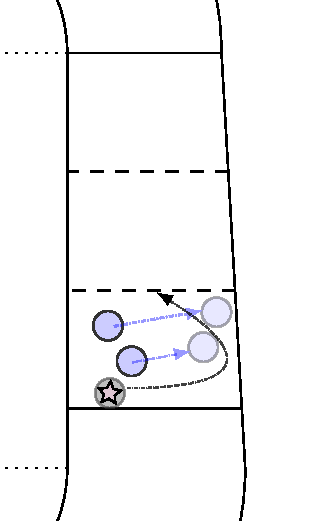
\includegraphics[scale=1.1,trim={0 0 0 4cm}, clip]{img/colinear_double_lines/escape}
{\it The approximate path of the jammer and blockers.}
\end{centering}

\end{minipage}
\hfill
\hspace{0.5cm}
\begin{minipage}{0.6\textwidth}


This drill involves a colinear two wall and a jammer.
There are four variations of this drill.

In rough order of difficult these are:
\begin{itemize}
\item Blocker in lane 1.5, brace in lane 1
\item Blocker in lane 3.5, brace in lane 4
\item Blocker in lane 1.5, brace in lane 2
\item Blocker in lane 3.5, brace in lane 3
\end{itemize} 


The jammer begins behind the rear blocker.

The goal of the jammer is to out-pace the wall to the other side of the track and pass the blockers in either lane 1 or lane 4.
The jammer must commit to this movement until they have passed the first blocker. 
\end{minipage}

\vspace{0.5cm}
\begin{minipage}{0.6\textwidth}

The goals of this drill vary depending on the level of the jammer and the blockers.

\begin{itemize}
\item The first goal is for the jammer to outpace the blockers sufficiently to escape.
\item The second is for the blockers to reach the line in time to prevent this. This will often involve the first blocker arriving too late, while the brace is in position to catch the jammer.
\item The third goal is for the jammer to avoid taking a double line and instead cut back into the seam.
\item Lastly, the blockers, after cutting off the line should close shoulders to prevent the jammer cutting through.
\end{itemize}
\end{minipage}
\hfill
\hspace{0.5cm}
\begin{minipage}{0.38\textwidth}
\begin{centering}
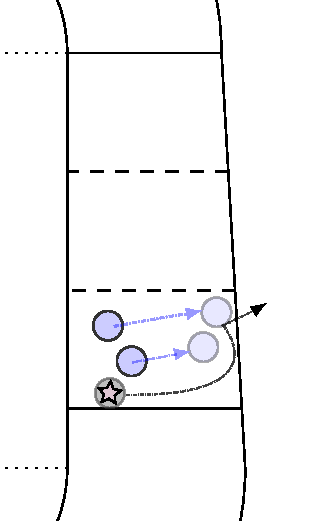
\includegraphics[scale=1.1,trim={0 0 0 4cm}, clip]{img/colinear_double_lines/caught}
{\it The jammer fails to cut back in and is caught or hit out.}
\end{centering}
\end{minipage}



% TODO Figure
